\documentclass{beamer}

\usepackage[utf8]{inputenc}
\usepackage[numbers,sort&compress]{natbib}
\usepackage{multirow}
\usepackage{booktabs}
\usepackage{float}
\usepackage{bbding}
\usepackage{array}
\usepackage{tikz}
\let\Tiny\tiny
\beamertemplatenavigationsymbolsempty

\usepackage{braket}
\usepackage{booktabs}
\usepackage{makecell}
\usepackage{multirow}
\usepackage{makecell}
\usepackage{slashed}
\usepackage{mdframed}
\usepackage{setspace}
\usepackage{tikz}
\usetheme{Madrid}

% Define custom WashU red color
\definecolor{WashURed}{RGB}{151,38,32}

% Use the custom color as the structure color
\usecolortheme[named=WashURed]{structure}

% Customize bullets and header
\setbeamercolor{item projected}{bg=WashURed, fg=white}
\setbeamercolor{frametitle}{fg=white}
\setbeamercolor{section in toc}{fg=WashURed}
\setbeamercolor{section in head/foot}{bg=WashURed, fg=white}
\setbeamercolor{subsection in head/foot}{bg=WashURed, fg=white}

% Fix only the title block background (not others)
\setbeamercolor{title}{fg=white, bg=WashURed}
\setbeamerfont{title}{size=\LARGE, series=\bfseries}

\renewcommand\qedsymbol{$\blacksquare$}
\newcommand{\be}{\begin{equation}}
\newcommand{\ee}{\end{equation}}
\newcommand{\bea}{\begin{eqnarray}}
\newcommand{\eea}{\end{eqnarray}}
\newcommand{\bi}{\begin{itemize}}
\newcommand{\ei}{\end{itemize}}
\newcommand{\ba}{\begin{aligned}}
\newcommand{\ea}{\end{aligned}}
\newcommand{\dst}{\displaystyle}
\newcommand{\fr}[2]{\frac{{\dst #1}}{{\dst #2}}}
\renewcommand{\Re}{\mathrm{Re }}
\renewcommand{\Im}{\mathrm{Im }}
%\renewcommand{\Ker}{\mathrm{Ker }}
\newcommand{\doublet}[2]{ \left( \begin{array}{c}#1 \\ #2 \end{array}\right) }
\newcommand{\bracket}[2]{ \langle #1|#2 \rangle}
\newcommand{\triplet}[3]{ \left(\! \begin{array}{c}#1 \\ #2 \\ #3 \end{array}\!\right) }
\providecommand{\mtrx}[1]{\begin{pmatrix} #1 \end{pmatrix}}
\newcommand{\lr}[1]{ \langle #1 \rangle}
\newcommand{\Tr}{\mathrm{Tr}}
\newcommand{\Z}{\mathbb{Z}}
\newcommand{\mmatrix}[4]{ \left(\! \begin{array}{ccc}#1 & #2 \\ #3 & #4 \end{array}\!\right) }
\newcommand{\mmmatrix}[9]{ \left(\!\! \begin{array}{ccc}#1 & #2 & #3\\ #4 & #5 & #6\\ #7 & #8 & #9\\ \end{array}\!\!\right) }
\providecommand{\id}{{\boldsymbol{1}}}
\newcommand{\diag}{\mathrm{diag}}
\newcommand{\Aut}{\mathrm{Aut}}
\newcommand{\Ker}{\mathrm{Ker}}
\newcommand{\fdf}[2]{(\phi^\dagger_{#1}\phi_{#2})}
\newcommand{\fdfn}[2]{\phi^\dagger_{#1}\phi_{#2}}

\newcommand{\blue}{\color{blue}}
\definecolor{darkred}{rgb}{0.7,0.0,0.0}
\newcommand{\red}{\color{WashURed}}
\newcommand{\gray}{\color{gray}}
\definecolor{darkgreen}{rgb}{0.0,0.5,0.0}
\newcommand{\green}{\color{darkgreen}}

\newcommand{\setfootlabel}[1]{\def\insertshorttitle{#1}}

\def\lsim{\mathrel{\rlap{\lower4pt\hbox{\hskip1pt$\sim$}}
\raise1pt\hbox{$<$}}}         %less than or approx. symbol
\def\gsim{\mathrel{\rlap{\lower4pt\hbox{\hskip1pt$\sim$}}
\raise1pt\hbox{$>$}}}         %greater than or approx. symbol
%%%%%%%%%%%%%%%%%%%%%%%%%%%%%%%%%%%%%%%%%%%%%%%%%%%%%%%%%%%%%%%%%%%%%%%%
%%BEGINNING OF TEXT
%%%%%%%%%%%%%%%%%%%%%%%%%%%%%%%%%%%%%%%%%%%%%%%%%%%%%%%%%%%%%%%%%%%%%%%%


% Custom title page layout: only title block is red
\setbeamertemplate{title page}{
  \begin{centering}
    \vspace*{1cm}
    \begin{beamercolorbox}[sep=1em,center,rounded=true,shadow=true]{title}
      \usebeamerfont{title}\inserttitle\par
    \end{beamercolorbox}
    \vspace{0.5cm}
    {\usebeamerfont{author}\insertauthor\par}
    \vspace{0.3cm}
    {\usebeamerfont{institute}\insertinstitute\par}
    \vspace{0.3cm}
    {\usebeamerfont{date}\insertdate\par}
  \end{centering}
}

\title[NNPSS 2026]{Quark Matter Phase Boundary Evolution in Neutron Star Mergers}
\author[Jiazhen Shao]{Jiazhen Shao\textsuperscript{\dag}}
\institute[WashU]{
    {
\includegraphics[scale=0.22]{images/WashU_A&S_2.jpg}} \\
    {$^\dagger$\it Department of Physics, Washington University in St. Louis, School of Arts \& Sciences}
}
\date{\today}

% Top-right WashU logo on all slides
\addtobeamertemplate{frametitle}{}{%
  \begin{tikzpicture}[remember picture,overlay]
    \node[anchor=north east,yshift=6pt, xshift=7pt] at (current page.north east)
      {
\includegraphics[scale=0.11]{images/WashU.png}};
  \end{tikzpicture}
  \vspace{-10pt}
}



\begin{document}

\begin{frame}
\titlepage
\end{frame}








%------------------------------------------------------------
% Frame 1: QCD Phase Diagram
%------------------------------------------------------------
\begin{frame}
\frametitle{The QCD Phase Diagram}

\begin{columns}[c]
  \column{0.60\linewidth}
  \centering
  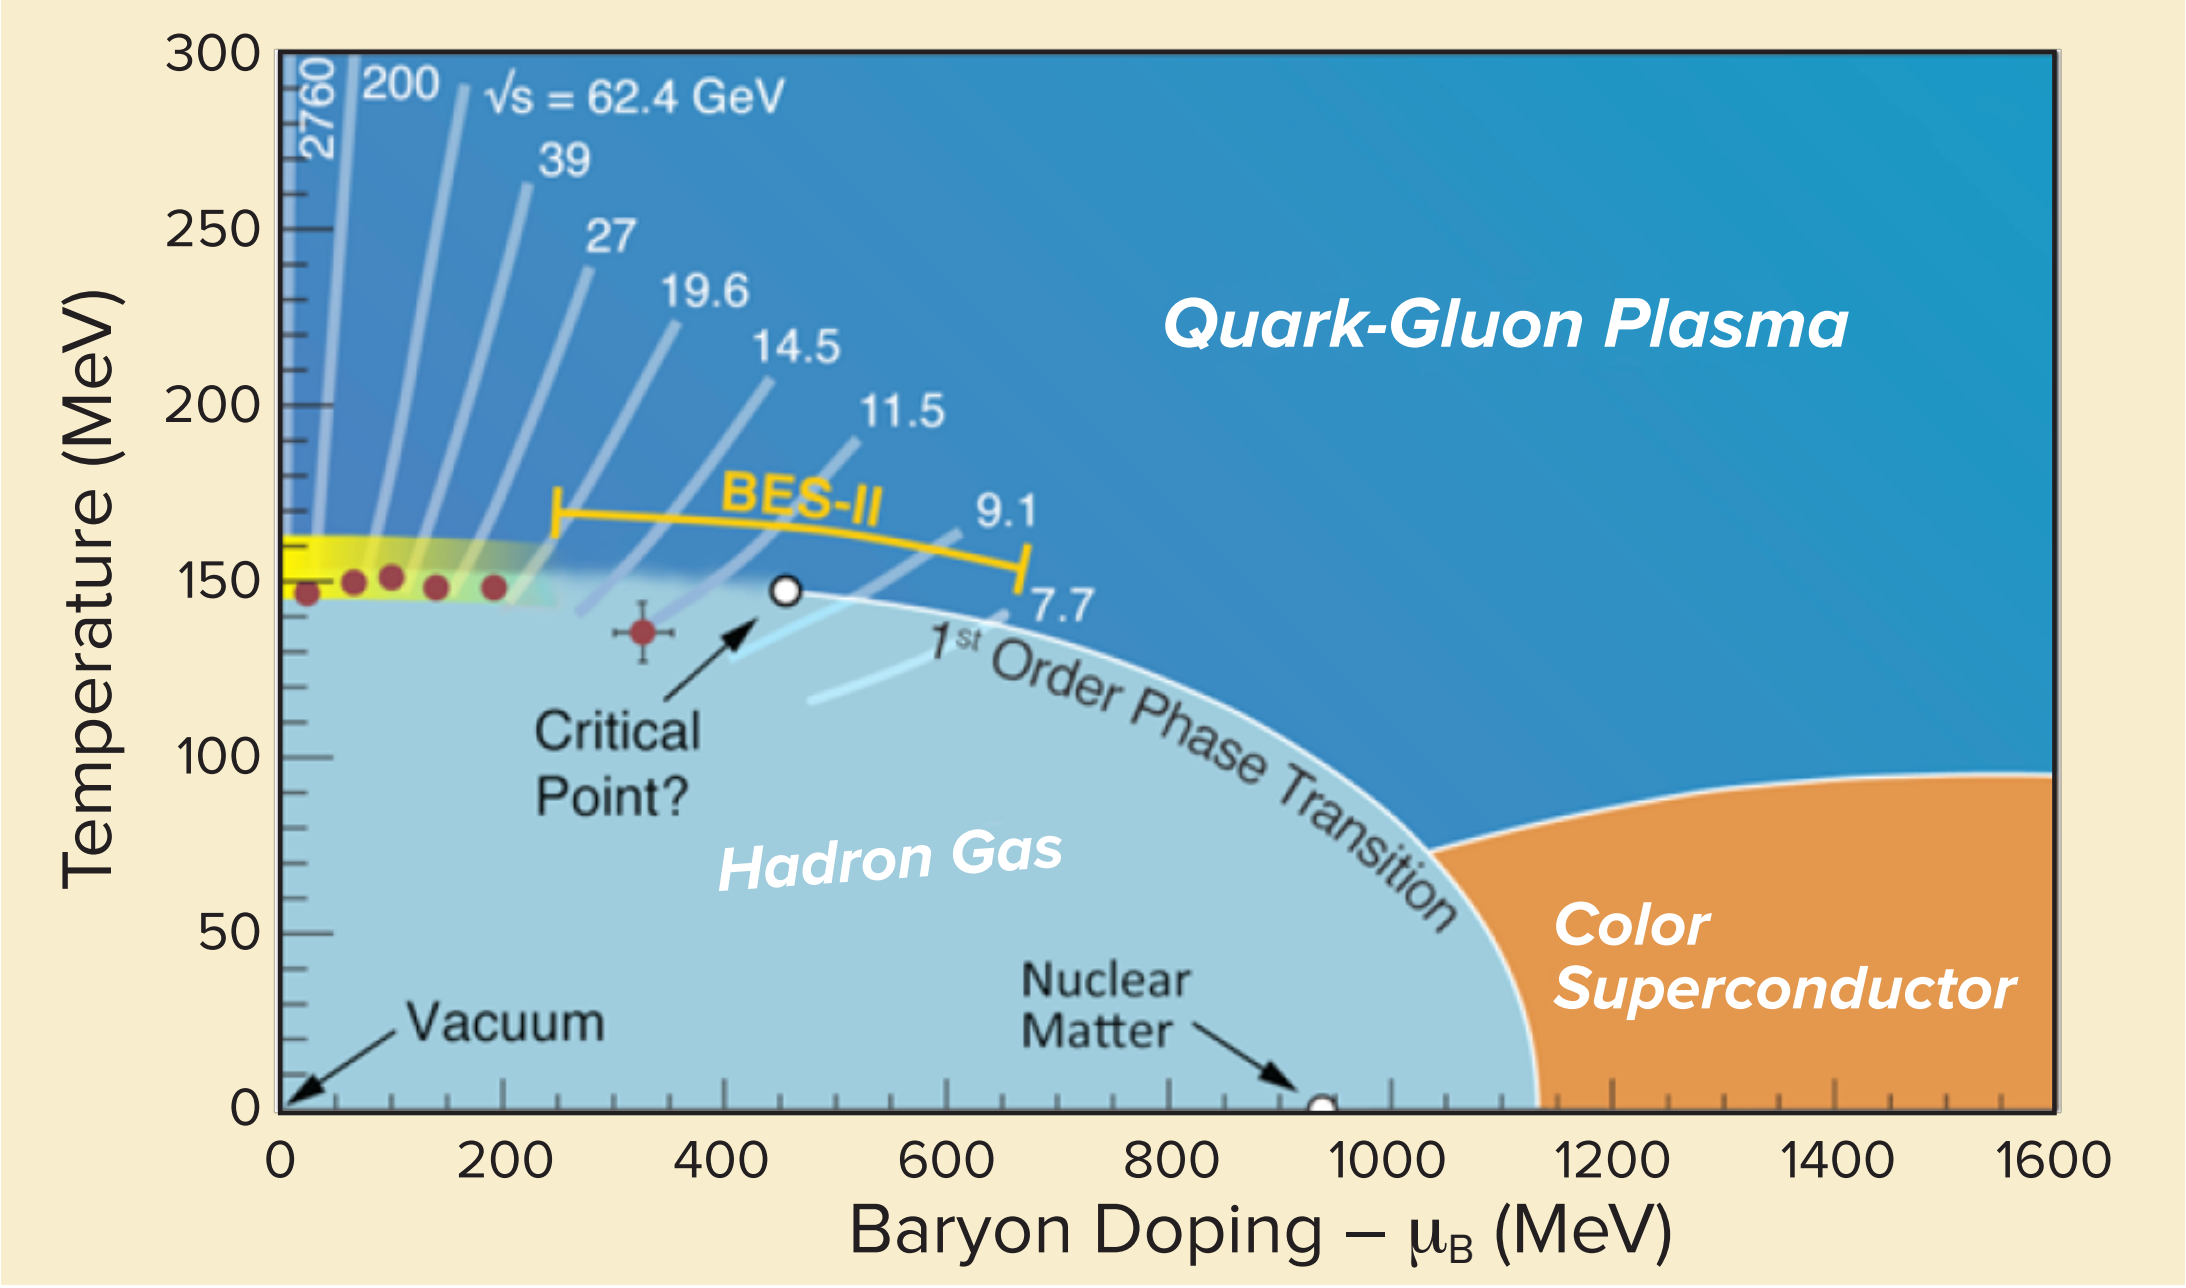
\includegraphics[width=\linewidth]{images/QCD-Phase-Diagram.png}

  \column{0.40\linewidth}
  \raggedright
  \textbf{Two very different regimes:}
  \vspace{0.5em}
  \bi
    \item \textbf{High $T$, low $\mu_B$}\\
          Quark-gluon plasma — explored at RHIC, LHC\\[0.2em]
          {\footnotesize$\to$ the compelling frontier $\sim$20 years ago}
    \vspace{0.5em}
    \item \textbf{Low $T$, high $\mu_B$ (${\sim}1\,\text{GeV}$)}\\
          Dense cores of neutron stars\\[0.2em]
          {\footnotesize$\to$ few experimental handles — until now}
  \ei
\end{columns}

\end{frame}


%------------------------------------------------------------
% Frame 2: Why Now + Research Question
%------------------------------------------------------------
\begin{frame}
\frametitle{Why Now? Multi-Messenger Astronomy}

%\textbf{Then:} high-$T$, low-$\mu_B$ was the frontier (collider experiments)
%
%\vspace{0.6em}
%\textbf{Now:} a new window onto low-$T$, high-$\mu_B$ matter
%\bi
%  \item Gravitational waves (LIGO/Virgo/KAGRA) from neutron-star mergers
%  \item Neutrino signals from core collapse/neutron-star mergers (IceCube, Hyper-Kamiokande, DUNE)
%  \item[$\Rightarrow$] Both directly probe $T\!\sim\!10\text{--}100\,\text{MeV}$,\; $\mu_B\!\sim\!1\,\text{GeV}$
%\ei
%
%\vspace{0.5em}

\textbf{Open question:} Is there a 1\textsuperscript{st}-order phase transition\\
\hspace{2.7em} between nuclear matter and quark matter at low $T$?

\vspace{0.5em}
\textbf{Strategy:} assume yes $\;\Rightarrow\;$ what is the \textbf{GW signature}\\
\hspace{3.5em} of such a transition in a merger?

\vspace{0.5em}
{\red$\Rightarrow$ Most important dynamical quantity: the \textbf{phase boundary velocity}}

\end{frame}


%------------------------------------------------------------
% Frame 3: Physical Picture
%------------------------------------------------------------
\begin{frame}
\frametitle{Nuclear-to-Quark-Matter Conversion Front}

\noindent
\begin{minipage}[t]{0.54\linewidth}
\raggedright
\textbf{Setup:} planar steady front propagating at velocity $u_N$
\vspace{0.4em}
\bi
  \item \textbf{Upstream} ($x\to-\infty$): nuclear matter (NM)\\
        density $n_B^N$, temperature $T_N$, chemical potential $\mu_B^N$
  \item \textbf{Downstream} ($x\to+\infty$): strange quark matter (QM)\\
        with ``K'' density $n_K = \tfrac{1}{2}(n_d{-}n_s)$, equilibrated when $\mu_K{=}0$
  \item Key parameters: bag constant $B^{1/4}$, strong coupling $\alpha_s$
\ei
\vspace{0.4em}
{\small EOS: RMF (QMC-RMF3)~\cite{Alford:2022bpp,Alford:2023rgp} for NM \;$|$\; bag model~\cite{Farhi:1984qu} for QM}
\end{minipage}
\hfill
\begin{minipage}[t]{0.44\linewidth}
\raggedright
\vspace{0.3em}
\begin{center}
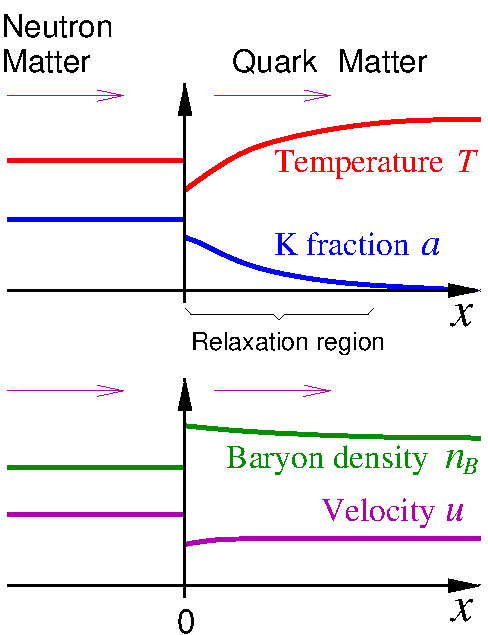
\includegraphics[width=\linewidth]{images/boundary_schematic.pdf}
\end{center}
\vspace{0.3em}
{\footnotesize Prior hydro studies: \cite{Niebergal:2010ds,Furusawa:2015vfn}}
\end{minipage}

\end{frame}


%------------------------------------------------------------
% Frame 4: Hydrodynamic Framework
%------------------------------------------------------------
\begin{frame}
\frametitle{Relativistic Hydrodynamics Across the Front}

Steady 1-D front: conservation laws must hold across the interface.

\vspace{0.5em}
\textbf{Fluxes conserved :}\qquad  $\partial_\mu T^{\mu\nu} = 0\,,\quad  \partial_\mu (n_B U^\mu) = 0$
\bea
j_B &=& n_B\,u \;=\; \text{const} \quad \text{(baryon current)} \nonumber\\
\Pi  &=& h\,u^2 + P \;=\; \text{const} \quad \text{(momentum flux)} \nonumber\\
\mathcal{E} &=& h\,u\,\gamma \;=\; \text{const} \quad \text{(energy flux)} \nonumber
\eea

\vspace{0.3em}
\textbf{K production ODE} (strangeness-changing weak interaction~\cite{Madsen:1993xx}):
\[
j_K \equiv n_K\,u - D_K\frac{dn_K}{dx}, \qquad \frac{dj_K}{dx} = \Gamma_K(\mu_u,\,\mu_K,\,T)
\]

\textbf{Boundary conditions:}
\bi
  \item $x\to-\infty$: NM in $\beta$-equilibrium, $n_K = 0$
  \item $x\to+\infty$: QM with $\mu_K = \mu_d - \mu_s = 0$
\ei

%Solved as a \textbf{boundary-value problem} (shooting method, \texttt{scipy.integrate.solve\_bvp}).

\end{frame}


%------------------------------------------------------------
% Frame 4: Results — Analytic Velocity Bound
%------------------------------------------------------------
\begin{frame}
\frametitle{Front Velocity in Parameter Space}

\begin{center}
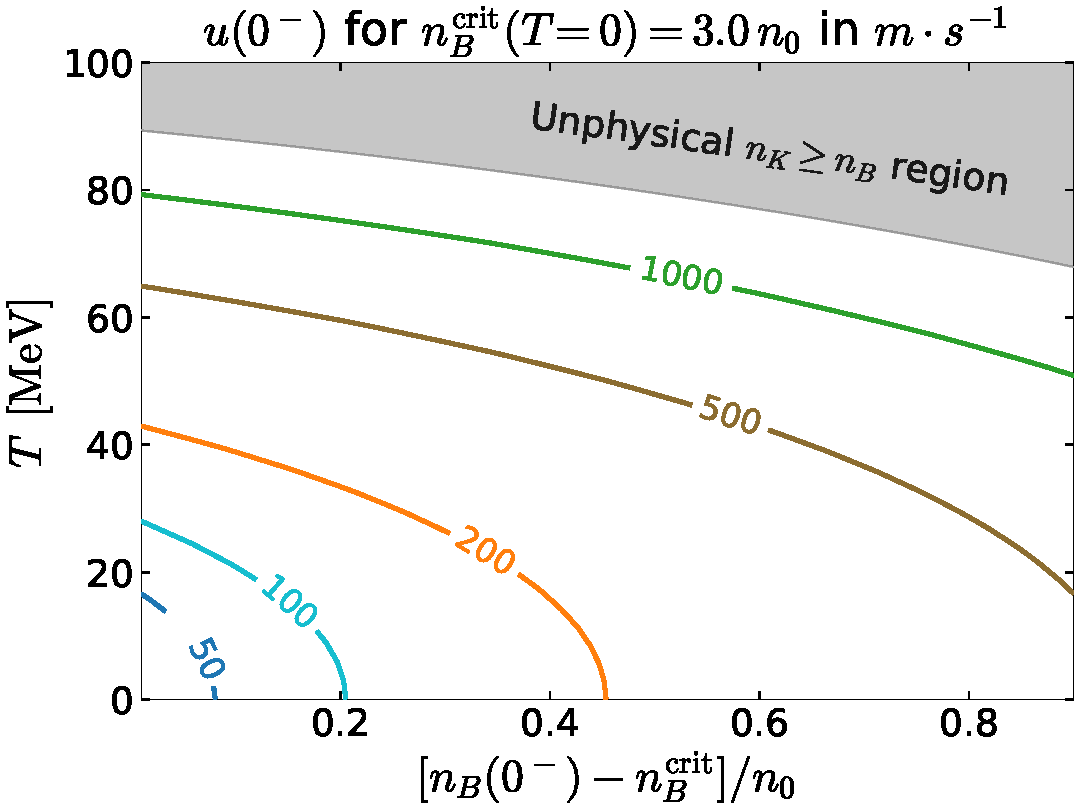
\includegraphics[width=0.88\linewidth]{images/uNmax-numerical-contour.pdf}
\end{center}

\end{frame}


%------------------------------------------------------------
% Frame 5: Summary
%------------------------------------------------------------
\begin{frame}
\frametitle{Summary}

\bi
  \item[\checkmark] Solved for \textbf{steady planar NM$\to$QM conversion fronts} from first principles
  \vspace{0.3em}
  \item[\checkmark] \textbf{Relativistic hydro conservation} (baryon, momentum, energy) coupled with \textbf{weak-interaction K production} in a unified BVP framework
  \vspace{0.3em}
  \item[\checkmark] Front velocity mapped as a function of $(T,\,n_B,\,B^{1/4})$ — bounded by hydro closure and weak timescale $\tau_{\rm weak}$
  \vspace{0.3em}
  \item[$\square$] Collaborate with merger simulation community to get $f_{\rm peak}$ and maximum strain etc. %Results relevant for \textbf{neutron-star merger} post-merger dynamics, gravitational-wave signatures, and nucleosynthesis
\ei

%\vspace{0.8em}
%\begin{center}
%{\small Work in preparation: \textit{Quark Matter Phase Boundary Evolution in Neutron Star Mergers}}
%\end{center}

\end{frame}


% Thank you page
\begin{frame}
\vspace{1.5em}
\Huge{\centerline{Thank you!}}
\vspace{1.5em}

{\normalsize
\begin{center}
{Work in collaboration with:}\\[0.5em]
M.~G.~Alford$^{1}$\,,\quad
L.~Brodie$^{1}$\,,\quad
A.~Haber$^{1,2}$\\
\vspace{0.8em}
{\small\it $^1$Department of Physics, Washington University in St.\ Louis}\\
{\small\it $^2$Mathematical Sciences \& STAG Research Centre, University of Southampton}\\
\end{center}
}

\end{frame}


\bibliography{references}
\bibliographystyle{unsrt}

\end{document}